\documentclass[a4paper,12pt]{article}

\usepackage{a4wide}
\usepackage{amsfonts}
\usepackage{amsmath}
\usepackage{amssymb}
\usepackage{csquotes}
\usepackage{lipsum}
\usepackage{bm}
\usepackage{tabularx}
\usepackage{longtable}
\usepackage{booktabs}
\usepackage{array}
\usepackage{tikz}
\usepackage{float}
\usetikzlibrary{positioning, arrows.meta, shapes.geometric, fit}

\usepackage{graphicx}  % For including images
\usepackage{xcolor}  % For a colorfull presentation
\usepackage{listings}  % For presenting code 

\usepackage{algorithm}
\usepackage[noend]{algpseudocode}
\makeatletter
\def\BState{\State\hskip-\ALG@thistlm}
\makeatletter
\usepackage[normalem]{ulem}
\usepackage{array}
\usepackage{hyperref}
% \usepackage[hyphens]{url}

\hypersetup{
  colorlinks=true,
  linkcolor=blue,
  urlcolor=blue,
  citecolor=blue
}
\newcommand{\bluehref}[2]{\href{#1}{\textcolor{blue}{\uline{#2}}}}
\makeatletter
\newcommand*{\citelinktext}[2]{%
  \hyper@@link[cite]{}{cite.#1}{#2}}
\makeatother

\usepackage{booktabs} 
\usepackage{enumitem}
\usepackage{bbm}
\usepackage{tcolorbox}

\usepackage{minted}
\usepackage{subcaption}

\usepackage[font=small,labelfont=bf]{caption}

\usepackage{fullpage,amsmath,amsthm,amssymb}
\newtheorem*{solution}{Solution}
\newtheorem*{part1}{Part 1}
\newtheorem*{part2}{Part 2}

\newcommand{\Cov}{\mathrm{Cov}}
\newcommand{\Var}{\mathrm{Var}}
\newcommand{\rank}{\mathrm{rank}}
\newcommand{\Span}{\mathrm{span}}
\newcommand{\clip}{\mathrm{clip}}
\newcommand{\Dim}{\mathrm{dim}}

\newcolumntype{Y}{>{\raggedright\arraybackslash}X}
\newcolumntype{R}[1]{>{\raggedright\arraybackslash}p{#1}}

\tcbset{
  colback=gray!3,
  colframe=black!20,
  boxsep=1mm,
  left=1mm,
  right=1mm,
  top=1mm,
  bottom=1mm,
}

\usepackage{changepage}
\newenvironment{restoretext}%
    {
     \begin{adjustwidth}{}{\leftmargin}%
    }{\end{adjustwidth}
     }

% Definition of a style for code, matter of taste
\lstdefinestyle{mystyle}{
  language=Python,
  basicstyle=\ttfamily\footnotesize,
  backgroundcolor=\color[HTML]{F7F7F7},
  rulecolor=\color[HTML]{EEEEEE},
  identifierstyle=\color[HTML]{24292E},
  emphstyle=\color[HTML]{005CC5},
  keywordstyle=\color[HTML]{D73A49},
  commentstyle=\color[HTML]{6A737D},
  stringstyle=\color[HTML]{032F62},
  emph={@property,self,range,True,False},
  morekeywords={super,with,as,lambda},
  literate=%
    {+}{{{\color[HTML]{D73A49}+}}}1
    {-}{{{\color[HTML]{D73A49}-}}}1
    {*}{{{\color[HTML]{D73A49}*}}}1
    {/}{{{\color[HTML]{D73A49}/}}}1
    {=}{{{\color[HTML]{D73A49}=}}}1
    {/=}{{{\color[HTML]{D73A49}=}}}1,
  breakatwhitespace=false,
  breaklines=true,
  captionpos=b,
  keepspaces=true,
  numbers=none,
  showspaces=false,
  showstringspaces=false,
  showtabs=false,
  tabsize=4,
  frame=single,
}
\lstset{style=mystyle}

\begin{document}
\begin{titlepage}
    \centering
    \vspace*{1cm}
    
    \Huge
    \textbf{CSC490: Assignment 3}
    
    \vspace{0.5cm}
    
    \vspace{1.5cm}
    
    \textbf{Team Members}
    
    \vspace{0.8cm}
    
    \large
    \begin{tabular}{ll}
        \textbf{Name} & \textbf{Student ID} \\
        \midrule
        Aarya Prakash & 1008790257 \\
        Derek Huynh & 1008849052 \\
        Merrick Liu & 1008951920 \\
        Rhys Balevicius & 1000801974 \\
    \end{tabular}
    
    \vfill
    
    \large
    University of Toronto\\
    Department of Computer Science    
\end{titlepage}

\section{Architecture Review}

\subsection{Original \texttt{nanochat} Architecture (October 2023)}

The original \texttt{nanochat} (Oct 13) implemented a minimal decoder-only Transformer closely following the GPT-2 architecture \cite{radford2019language}:

\begin{itemize}
    \item Decoder-only Transformer
    \item Learned absolute positional embeddings
    \item Multi-Head Attention (MHA) — equal Q, K, V heads
    \item LayerNorm (with learnable scale and bias)
    \item GELU feedforward network: $\text{Linear} \rightarrow \text{GELU} \rightarrow \text{Linear}$
    \item Tied token embedding and output projection (\texttt{lm\_head})
    \item Standard full causal attention (no sliding window)
\end{itemize}

\subsection{Updated \texttt{nanochat} Architecture (February 2026)}

The February 2026 revision incorporates several improvements motivated by advances in LLM architecture research, the differences are:

\begin{itemize}
    \item Decoder-only Transformer
    \item Rotary Positional Embeddings (RoPE) \cite{su2024roformer} — replaces learned absolute embeddings
    \item Grouped Query Attention (GQA) \cite{ainslie2023gqa} — fewer K/V heads than Q heads
    \item RMSNorm \cite{zhang2019root} — replaces LayerNorm, no learnable bias
    \item ReLU$^2$ feedforward network \cite{so2022primer}: $\text{Linear} \rightarrow \text{ReLU}^2 \rightarrow \text{Linear}$
    \item Untied token embedding and output projection (\texttt{lm\_head})
    \item FlashAttention (FA3 where available, otherwise PyTorch SDPA) \cite{dao2023flashattention2}
    \item Sliding-window attention pattern across layers \cite{beltagy2020longformer}
    \item Value residual mechanism: $V \leftarrow V + \sigma(g(x)) \cdot \mathrm{VE}(x)$
    \item Per-layer learnable residual scaling parameters
\end{itemize}

\subsection{Architecture Diagrams}

\subsubsection{High-Level Model Architecture}

\begin{figure}[H]
\centering
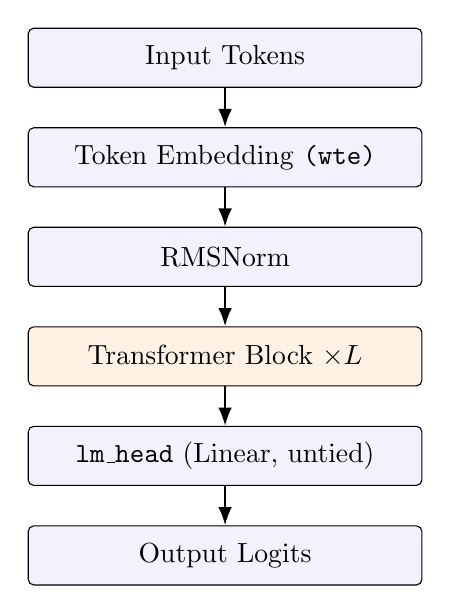
\begin{tikzpicture}[
    block/.style={draw, rectangle, rounded corners=2pt, minimum width=5cm,
                  minimum height=0.75cm, align=center, fill=blue!5},
    arrow/.style={-Latex, thick}
]
\node[block] (tokens) {Input Tokens};
\node[block, below=0.5cm of tokens] (embed) {Token Embedding \texttt{(wte)}};
\node[block, below=0.5cm of embed] (norm0) {RMSNorm};
\node[block, below=0.5cm of norm0, fill=orange!10] (block) {Transformer Block $\times L$};
\node[block, below=0.5cm of block] (lmhead) {\texttt{lm\_head} (Linear, untied)};
\node[block, below=0.5cm of lmhead] (logits) {Output Logits};

\draw[arrow] (tokens) -- (embed);
\draw[arrow] (embed) -- (norm0);
\draw[arrow] (norm0) -- (block);
\draw[arrow] (block) -- (lmhead);
\draw[arrow] (lmhead) -- (logits);
\end{tikzpicture}
\caption{High-level \texttt{nanochat} architecture (Feb 2026). The embedding and \texttt{lm\_head}
weights are \textbf{untied}, unlike the original Oct 13 model.}
\end{figure}

\subsubsection{Transformer Block Detail}

\begin{figure}[H]
\centering
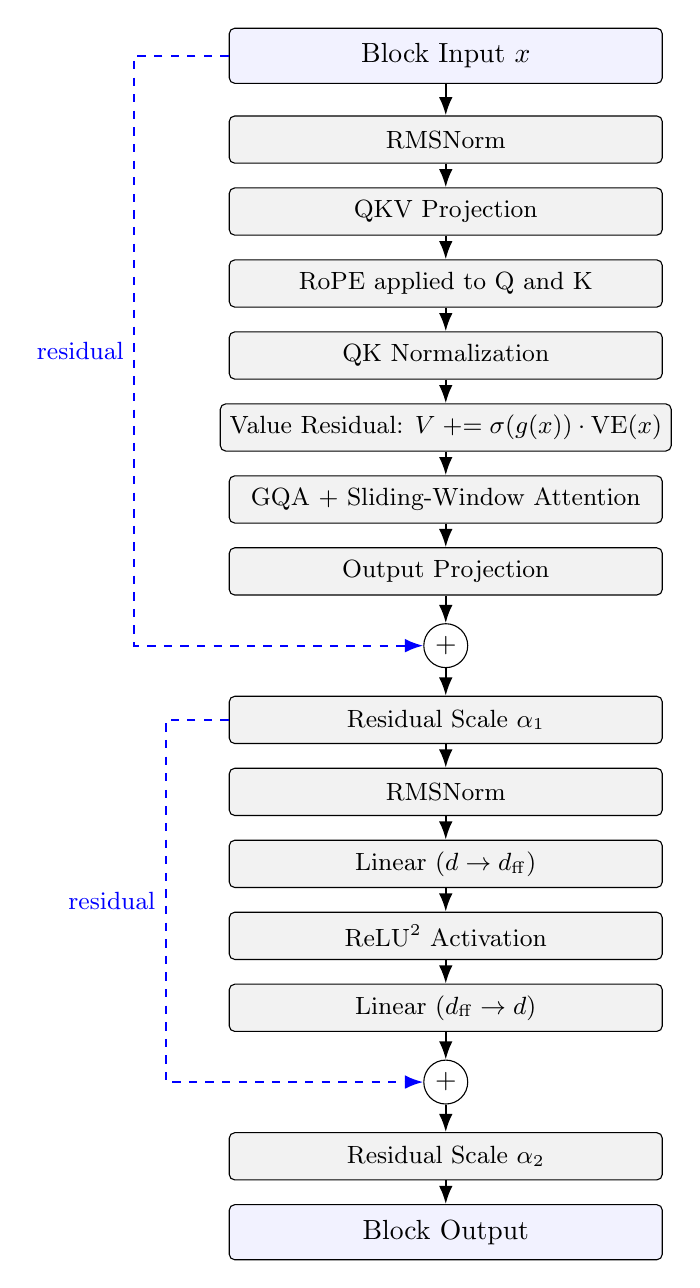
\begin{tikzpicture}[
    block/.style={draw, rectangle, rounded corners=2pt, minimum width=5.5cm,
                  minimum height=0.7cm, align=center, fill=blue!5},
    subblock/.style={draw, rectangle, rounded corners=2pt, minimum width=5.5cm,
                     minimum height=0.6cm, align=center, fill=gray!10, font=\small},
    arrow/.style={-Latex, thick},
    plus/.style={circle, draw, inner sep=2pt, font=\normalsize}
]

\node[block] (input) {Block Input $x$};
\node[subblock, below=0.4cm of input] (norm1) {RMSNorm};
\node[subblock, below=0.3cm of norm1] (qkv) {QKV Projection};
\node[subblock, below=0.3cm of qkv] (rope) {RoPE applied to Q and K};
\node[subblock, below=0.3cm of rope] (qknorm) {QK Normalization};
\node[subblock, below=0.3cm of qknorm] (vres) {Value Residual: $V \mathrel{+}= \sigma(g(x))\cdot\mathrm{VE}(x)$};
\node[subblock, below=0.3cm of vres] (attn) {GQA + Sliding-Window Attention};
\node[subblock, below=0.3cm of attn] (proj) {Output Projection};
\node[plus, below=0.35cm of proj] (add1) {$+$};
\node[subblock, below=0.35cm of add1] (scale1) {Residual Scale $\alpha_1$};
\node[subblock, below=0.3cm of scale1] (norm2) {RMSNorm};
\node[subblock, below=0.3cm of norm2] (ff1) {Linear ($d \rightarrow d_\mathrm{ff}$)};
\node[subblock, below=0.3cm of ff1] (relu2) {ReLU$^2$ Activation};
\node[subblock, below=0.3cm of relu2] (ff2) {Linear ($d_\mathrm{ff} \rightarrow d$)};
\node[plus, below=0.35cm of ff2] (add2) {$+$};
\node[subblock, below=0.35cm of add2] (scale2) {Residual Scale $\alpha_2$};
\node[block, below=0.3cm of scale2] (output) {Block Output};

\draw[arrow] (input) -- (norm1);
\draw[arrow] (norm1) -- (qkv);
\draw[arrow] (qkv) -- (rope);
\draw[arrow] (rope) -- (qknorm);
\draw[arrow] (qknorm) -- (vres);
\draw[arrow] (vres) -- (attn);
\draw[arrow] (attn) -- (proj);
\draw[arrow] (proj) -- (add1);
\draw[arrow] (add1) -- (scale1);
\draw[arrow] (scale1) -- (norm2);
\draw[arrow] (norm2) -- (ff1);
\draw[arrow] (ff1) -- (relu2);
\draw[arrow] (relu2) -- (ff2);
\draw[arrow] (ff2) -- (add2);
\draw[arrow] (add2) -- (scale2);
\draw[arrow] (scale2) -- (output);

% Residual connections on the LEFT to avoid overflow
\draw[arrow, dashed, blue] (input.west) -- ++(-1.2,0) |- (add1.west)
    node[pos=0.25, left, font=\small, blue] {residual};
\draw[arrow, dashed, blue] (scale1.west) -- ++(-0.8,0) |- (add2.west)
    node[pos=0.25, left, font=\small, blue] {residual};

\end{tikzpicture}
\caption{Detailed Transformer block for \texttt{nanochat} (Feb 2026). Dashed blue lines show
residual connections. Per-layer scalars $\alpha_1, \alpha_2$ modulate residual mixing.}
\end{figure}

\subsection{Key Changes: Oct 2023 $\rightarrow$ Feb 2026}

\begin{table}[H]
\centering
\small
\begin{tabular}{lll}
\toprule
\textbf{Component} & \textbf{Oct 13 (Original)} & \textbf{Feb 2026 (Current)} \\
\midrule
Positional Encoding & Learned absolute & RoPE \cite{su2024roformer} \\
Attention & Multi-Head (MHA) & Grouped Query (GQA) \cite{ainslie2023gqa} \\
Normalization & LayerNorm & RMSNorm \cite{zhang2019root} \\
Activation & GELU & ReLU$^2$ \cite{so2022primer} \\
Embedding & Tied & Untied \\
Attention Pattern & Full causal & Sliding-window \cite{beltagy2020longformer} \\
Attention Kernel & Standard & FlashAttention \cite{dao2023flashattention2} \\
Value Residual & None & Token-conditioned VE \\
Residual Scaling & None & Per-layer $\alpha$ scalars \\
\bottomrule
\end{tabular}
\caption{Architectural changes between the Oct 13 and Feb 2026 \texttt{nanochat} versions.}
\end{table}

\subsection{Proposed Architectural Improvements}

We propose three modifications grounded in recent literature to further improve the Feb 2026 \texttt{nanochat}.

\begin{longtable}{R{3.3cm} R{3.7cm} R{4.5cm} R{3.5cm}}
\toprule
\textbf{Proposed Change} & \textbf{Motivation} & \textbf{Technical Details} & \textbf{Expected Impact} \\
\midrule
\endfirsthead
\toprule
\textbf{Proposed Change} & \textbf{Motivation} & \textbf{Technical Details} & \textbf{Expected Impact} \\
\midrule
\endhead

Replace ReLU$^2$ FFN with SwiGLU &
GLU variants consistently outperform ReLU/GELU in language modelling. Used in LLaMA, PaLM, and Mistral. &
Replace:
$\text{Linear} \rightarrow \text{ReLU}^2 \rightarrow \text{Linear}$
with:
$y = (\text{SiLU}(xW_1) \odot xW_2)W_3$
Reduce $d_\mathrm{ff}$ by $\tfrac{2}{3}$ to preserve parameter count. &
Reported $\sim$0.5 PPL improvement at matched compute \cite{shazeer2020glu}. Better gradient flow through gating. \\
\midrule

Apply YaRN for RoPE Context Extension &
RoPE degrades sharply beyond trained sequence length. YaRN enables context extension with minimal retraining. &
Rescale rotary frequencies using NTK-aware interpolation with a ramp function. Optionally continue pretraining at target length (e.g., 8192 tokens) for $\sim$400M tokens. &
Recovers $>$99\% of performance at $8\times$ context extension. Near-zero architectural overhead \cite{peng2023yarn}. \\
\midrule

Global Tokens with Sliding-Window Attention &
Pure sliding-window attention cannot propagate information beyond the window, harming tasks requiring long-range dependencies. &
Prepend $G$ learned global tokens per layer. Local tokens attend locally + to all global tokens. Global tokens attend to the full sequence. Modify attention mask accordingly. &
Improved long-range coherence and summarisation. $O(n \cdot w + G \cdot n)$ complexity vs.\ $O(n^2)$ for full attention \cite{beltagy2020longformer, zaheer2020bigbird}. \\
\bottomrule
\caption{Proposed architectural improvements to the Feb 2026 \texttt{nanochat}.}
\label{tab:proposed_changes}\\
\end{longtable}

\subsection{Ablation Strategy}

To isolate the effect of each proposed change:

\begin{itemize}
    \item Modify one architectural component at a time against the Feb 2026 baseline.
    \item Hold constant: training tokens, batch size, learning rate schedule, and random seed.
    \item Evaluation metrics:
    \begin{itemize}
        \item Training and validation loss curves (tracked via Weights \& Biases)
        \item Validation perplexity
        \item Long-context perplexity at 2048, 4096, and 8192 tokens (for YaRN)
        \item Long-range dependency benchmarks (for global tokens)
    \end{itemize}
\end{itemize}

\newpage

\section{Ablations on a nano \texttt{nanochat}}

\newpage 

\section{Extending the Context Window}

\newpage

\section{Our Final \texttt{\texttt{nanochat}}}

\newpage 

\begin{thebibliography}{9}
\bibitem{radford2019language} Radford, A., et al. (2019). Language models are unsupervised multitask learners. OpenAI Blog.
\bibitem{su2024roformer} Su, J., et al. (2024). RoFormer: Enhanced transformer with rotary position embedding. \textit{Neurocomputing}, 568, 127063.
\bibitem{ainslie2023gqa} Ainslie, J., et al. (2023). GQA: Training generalized multi-query transformer models from multi-head checkpoints. \textit{arXiv:2305.13245}.
\bibitem{zhang2019root} Zhang, B., \& Sennrich, R. (2019). Root mean square layer normalization. \textit{NeurIPS}.
\bibitem{so2022primer} So, D., et al. (2022). Primer: Searching for efficient transformers for language modeling. \textit{NeurIPS}.
\bibitem{beltagy2020longformer} Beltagy, I., Peters, M. E., \& Cohan, A. (2020). Longformer: The long-document transformer. \textit{arXiv:2004.05150}.
\bibitem{dao2023flashattention2} Dao, T. (2023). FlashAttention-2: Faster attention with better parallelism and work partitioning. \textit{arXiv:2307.08691}.
\bibitem{shazeer2020glu} Shazeer, N. (2020). GLU variants improve transformer. \textit{arXiv:2002.05202}.
\bibitem{peng2023yarn} Peng, B., et al. (2023). YaRN: Efficient context window extension of large language models. \textit{arXiv:2309.00071}.
\bibitem{zaheer2020bigbird} Zaheer, M., et al. (2020). Big Bird: Transformers for longer sequences. \textit{NeurIPS}.
\end{thebibliography}
\end{document}
